\documentclass[12pt,letterpaper]{article}
\usepackage{natbib}

%Packages
\usepackage{textcomp}
\usepackage{fullpage}
\usepackage{float}
\usepackage{latexsym}
\usepackage{url}
\usepackage{epsfig}
\usepackage{graphicx}
\usepackage{amssymb}
\usepackage{amsmath}
\usepackage{mathtools}
\usepackage{bm}
\usepackage{array}
\usepackage[version=3]{mhchem}
\usepackage{ifthen}
\usepackage{caption}
\usepackage{hyperref}
\usepackage{amsthm}
\usepackage{amstext}
\usepackage{enumerate}
\usepackage[osf]{mathpazo}
\usepackage{dcolumn}
\usepackage{lineno}
\usepackage{pdflscape}

\usepackage{color,soul}

\DeclarePairedDelimiter\abs{\lvert}{\rvert}%
\DeclarePairedDelimiter\norm{\lVert}{\rVert}%
\newcolumntype{d}[1]{D{.}{.}{#1}}

\pagenumbering{arabic}


%Pagination style and stuff
\linespread{2}
\raggedright
\setlength{\parindent}{0.5in}
\setcounter{secnumdepth}{0} 
\renewcommand{\section}[1]{%
\bigskip
\begin{center}
\begin{Large}
\normalfont\scshape #1
\medskip
\end{Large}
\end{center}}
\renewcommand{\subsection}[1]{%
\bigskip
\begin{center}
\begin{large}
\normalfont\itshape #1
\end{large}
\end{center}}
\renewcommand{\subsubsection}[1]{%
\vspace{2ex}
\noindent
\textit{#1.}---}
\renewcommand{\tableofcontents}{}
%\bibpunct{(}{)}{;}{a}{}{,}

%---------------------------------------------
%
%       START
%
%---------------------------------------------

\begin{document}
%Running head
\begin{flushright}
Version dated: \today
\end{flushright}

\bigskip
\noindent RH: disparate disparity analyses
\bigskip
\medskip
\begin{center}
\noindent{\Large \bf Disparities in the analysis of morphological disparity}
\bigskip

Thomas Guillerme$^{1,16,*,+}$,
Natalie Cooper$^{2,+}$,
Stephen L. Brusatte$^{3}$,
Katie E. Davis$^{4}$,
Andrew L Jackson$^{5}$,
Sylvain Gerber$^{6}$,
Anjali Goswami$^{2}$,
Kevin Healy$^{7}$,
Melanie Hopkins$^{8}$,
Marc EH Jones$^{9}$,
Graeme T. Lloyd$^{10}$,
Joseph E. O'Reilly$^{11}$,
Abi Pate$^{11}$,
Mark N Puttick$^{12}$,
Emiliy Rayfield$^{11}$,
Erin E. Saupe$^{13}$,
Emma Sherratt$^{14}$,
Graham Slater$^{15}$,
Vera Weisbecker$^{1}$,
Gavin H Thomas$^{16}$
and Philip Donoghue$^{11}$\\


\noindent {\small \it 
$^1$School of Biological Sciences, University of Queensland, St. Lucia, Queensland, Australia;
$^2$IDepartment of Life Sciences, Natural History Museum, London, Cromwell Road, London, SW7 5BD, UK;
$^{3}$School of GeoSciences, University of Edinburgh, Grant Institute, Edinburgh EH9 3FE, UK;
$^{4}$Department of Biology, University of York, YO10 5DD, UK;
$^{5}$Department of Zoology, School of Natural Sciences, Trinity College, Ireland;
$^{6}$Institut de Syst\'{e}matique, \'{E}volution, Biodiversit\'{e} (ISYEB), Muséum national d'Histoire naturelle, CNRS, Sorbonne Universit\'{e}, EPHE, Université des Antilles, 57 rue Cuvier CP39, 75005 Paris, France;
$^{7}$Ryan Institute, School of Natural Sciences, National University of Ireland Galway, Ireland;
$^{8}$ @@@;
$^{10}$School of Earth and Environment, University of Leeds, Leeds LS2 9JT, UK;
$^{11}$School of Earth Sciences, University of Bristol, Life Sciences Building, Tyndall Avenue, Bristol BS8 1TQ, UK;
$^{12}$Milner Centre for Evolution, University of Bath, BA2 7AY UK;
$^{13}$Department of Earth Sciences, University of Oxford, S Parks Road, Oxford OX1 3AN, UK;
$^{14}$School of Biological Sciences, The University of Adelaide, Adelaide, South Australia 5005, Australia.
$^{15}$ @@@;
$^{16}$ @@@;\\
$^{+}$ These authors contributed equally to the manuscript; $^{*}$ Corresponding author: guillert@tcd.ie\\}

\end{center}

\textbf{Abstract (200 words max)}

\noindent Analyses of morphological disparity have been used to characterise and investigate the evolution of variation in the anatomy, function, and ecology of organisms since the 1980s.
While a diversity of methods have been employed, it is unclear whether they provide
equivalent insights.
Here we review the most commonly used approaches for characterising and analysing morphological disparity, all of which have associated limitations that, if ignored, can lead to misinterpretation.
We provide best practice guidelines for disparity analyses, while noting that there can be no ``one-size-fits-all'' approach.
The available tools should always be used in the context of a specific biological question that will determine data and method selection at every stage of the analysis.

\textbf{Keywords}: multidimensionality, palaeobiology, ecology,
morphology, disparity, variance/variation

\section{Introduction}

\noindent Clades of organisms are characterised by variation in both numbers of species and range of phenotypes through time.
At the extremes, clades may be exceptionally species-rich and phenotypically diverse (e.g. cichlids and molluscs), species-rich but phenotypically conservative (e.g. bacteria and nematodes), species-poor but phenotypically diverse (e.g. Afrotheria), or depauperate in both species and phenotypic diversity (e.g. lungfish).
These phenomena suggest that taxonomic and phenotypic diversity are not inextricably linked, raising important questions about how phenotypic diversity arises, such as:
How does diversity evolve?
Are some morphologies more common than others?
Can anatomy evolve in all ``directions'' or are some anatomies impossible to achieve? (Mike Foote 1997, 1995)
What role does ecology play in structuring morphological diversity?
Analyses of species diversity have a venerable history, but those of phenotypic diversity (hereafter \emph{disparity}) are a comparatively more recent phenomenon. Originally defined as ``multidimensional morphological dissimilarity at a macroevolutionary scale'' \citep{runnegar1987rates,Gould1991-nh} this concept of disparity emerged from attempts by palaeobiologists to characterise the evolutionary origin of animal bodyplans and from attempts by comparative developmental biologists to provide causal explanations for their emergence.
However, analyses of ``disparity'' have since expanded into comparative biology as a means of capturing the effect of intrinsic and extrinsic causal agents in morphological evolution.
Typically, methods to capture disparity are based on multidimensional spaces where each dimension represents an aspect of morphological variation (a trait) and biological observations (taxa) can be placed in this space based on their trait values.
Such multidimensional spaces (or morphospaces) can then be used to tackle a diverse array of questions that can be grouped into four main (non-mutually exclusive) classes (Fig. 1):

\begin{enumerate}

	\item \textbf{Descriptive disparity} The pioneering studies of disparity characterised the shapes of organisms and how they differed among groups \citep{Foote1995-do, Briggs1992-pd}.
	These studies consist of describing multidimensional patterns in the diversity of morphological traits, addressing questions such as: why are some morphological trait combinations more common than others and what are the biological (or mathematical) properties of the resulting morphospace? \citep{Foote1995-do, Raup1961-vx, Gerber2017-xi}.

	\item \textbf{Disparity-through-time} This approach investigates how the morphologies of organisms have changed on a temporal scale, focussing on the disparity of taxa in particular time intervals or slices.
	This approach has been used widely in palaeobiology to answer a range of macroevolutionary questions, such as: how does disparity accumulate over the history of a clade \citep{Guillerme2018-uj, Wright2017-jo}, or how does disparity change leading up to and across mass extinction events \citep{Friedman2010-ve}?

	\item \textbf{Disparity and taxonomic diversity} Morphological disparity provides another perspective on biodiversity; high morphological disparity represents a high diversity of morphologies (i.e. shapes or body plans) and is, presumably, associated with high levels of ecological and functional diversity (though see section 4 below).
	This makes disparity an informative complement to diversity measures based on species richness alone. Indeed, most studies that have investigated disparity and taxonomic diversity support an effective decoupling 
	\citep[][e.g.]{Fortey1996-kt, Moyne2007-jm, Ruta2013-iy, Hopkins2013-xt}.
	This approach has been used to investigate whether some groups are more successful than others in their exploration of new evolutionary strategies \citep{Losos2011-fq}.

	\item \textbf{Disparity as a proxy for ecology} The disparity of a group can be used as a proxy for either the functional role it plays within an ecosystem or its ecological niche.
	This approach assumes that groups with high disparity are also likely to be functionally and ecologically diverse, and that groups found in similar regions of shape space will have similar functional and ecological roles
	\citep{Friedman2010-ve, Pierce2008-yr, Anderson2013-zt}.
	The links between form and function, however, are not always clear cut.
	Traits can be linked to multiple functions and multiple functions can be linked to a single trait \citep{Wainwright2005-or}.
	This approach has been used to investigate hypotheses of competitive replacement \citep{Brusatte2008-vx} and changes in ecosystem function during and after mass extinctions \citep{Friedman2010-ve}.
	It is particularly common in palaeobiology where it is not possible to directly observe the ecological or functional characteristics of extinct species \citep{Wainwright2005-or}.

	\item \textbf{Disparity and evo-devo} Morphological disparity blalbalbal
% AG: Although intrinsic constraints are mentioned earlier, it doesn’t enter into any of these topics explicitly, but it is certainly one of the most interesting things one can use disparity for – to bridge development and evolution, looking at developmental biases/constraints. This also includes integration and modularity, which are also central to the topic of disparity and evolvability. Although you touch on these in places, I think it's really important to incorporate it into one of these topics, as there probably isn't room to give it one of its own (although i would argue it warrants equal footing with ecology, given that these are the processes that generate variation in the first place). There is a massive literature on using disparity to test hypotheses of developmental constraints, and also a huge one on disparity and integration/modularity. Let me know if you want me to send you refs.

\end{enumerate}

Fundamental insights into evolutionary biology have been elicited from these five types of analysis.
One of the most important insights is the discovery that morphological disparity is often greatest early in the evolutionary history of clades \citep{Foote1997-nl, Erwin2007-jz, Hughes2013-td}, indicating that the capacity for evolutionary innovation wanes with clade age, which some have argued reflects the evolutionary assembly of gene regulatory networks that constrain later fundamental change  \citep{Erwin2007-jz, Hughes2013-td}.
However, this example highlights one of the most challenging problems confronting researchers who are attempting, increasingly, to obtain general insights from multiple independent studies: can the insights gained from studies using the diversity of methods, approaches and data types employed be considered equivalent?

In attempting to answer this question, we review current methods and highlight their limitations, as part of a more general attempt to propose best practice guidelines for studies of disparity.
We first discuss the appropriate data required for characterising disparity, then review various challenging aspects of these approaches.
Throughout, it is important to remember these tools should always be used in the context of a specific scientific question, as this will drive data and methodological choices at every stage of the process.

%\includegraphics[width=6.5in,height=4.94444in]{media/image1.png}

\begin{figure}[!htbp]
\centering
   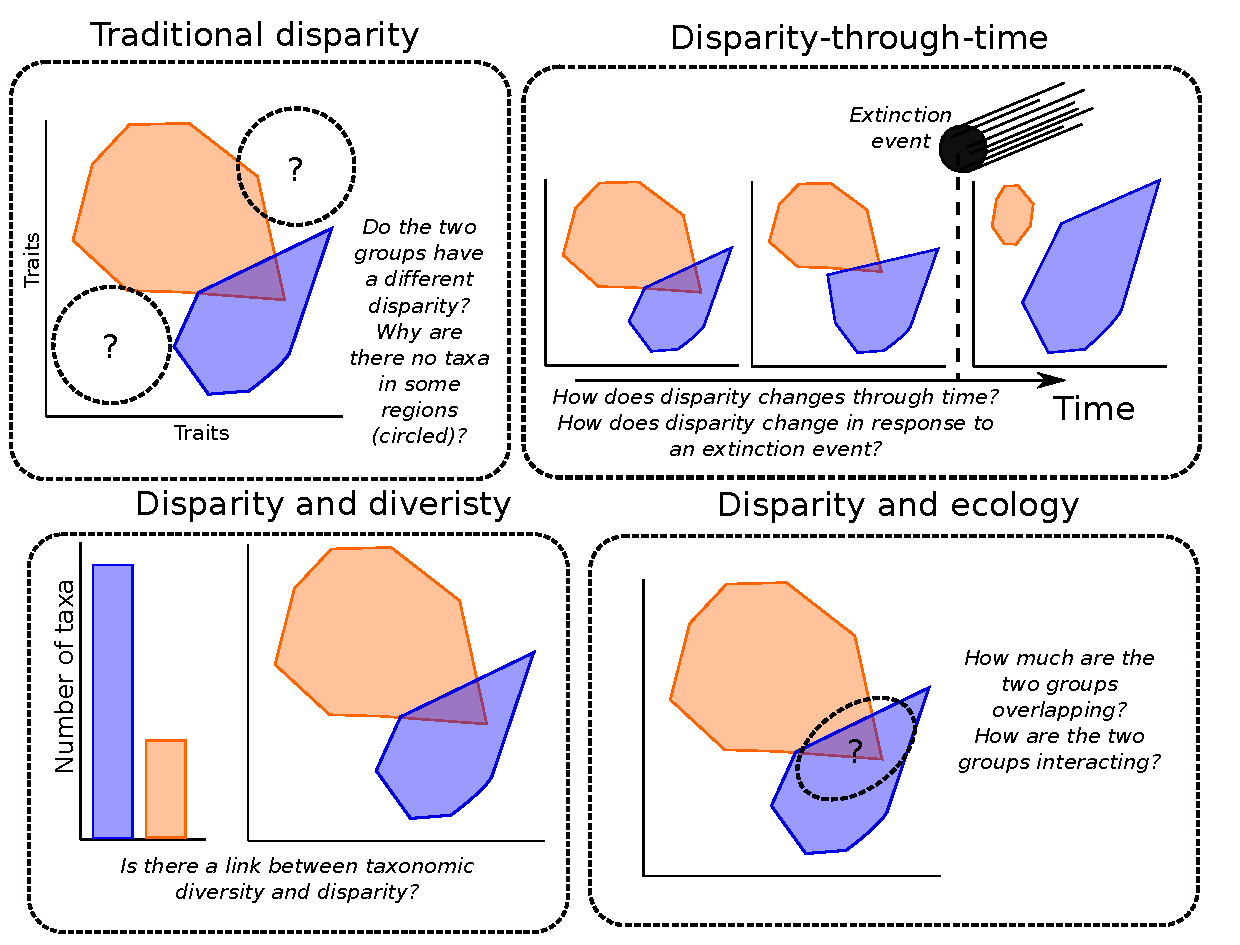
\includegraphics[width=0.9\textwidth]{Figures/figure_disparities.pdf}
\caption{
    The four main types of disparity analysis. \textbf{Descriptive disparity} focuses on describing the features of morphospace occupation; \textbf{disparity-through-time} investigates the evolution of the morphospace through time including the effect of extinction events; \textbf{disparity and taxonomic diversity} compares different measures of biodiversity ; \textbf{disparity as a proxy for ecology} uses disparity as a proxy for the ecological or functional role of a group.
    These categories are not independent and many disparity studies will cover more than one.
    %@@@ Add disparity and evo-devo
}
\label{Fig:disparity}
\end{figure}



\section{Data and disparity}

\noindent Disparity analyses are based on traits, but traits can be characterised in a number of ways:
% MH: We do not mention model-based descriptors at all, or the spaces defined by them (e.g. Raup's shell coiling models). I'm not convinced that we must, but it may come across as an notable omission to reviewers
% SG: I agree. There's for instance Saunders et al. (2004) disparity study of Paleozoic ammonoids using Raup's shell coiling parameters
	1) discrete ``cladistic'' characters, e.g. coding the absence or presence of features or a discrete characteristic of a trait \citep[][e.g]{Close2015-qi};
	2) continuous measurements of features (e.g., lengths) \citep[][e.g]{Anderson2001-qb}; or
	3) more mathematical descriptors from geometric morphometric landmark data (e.g. Procrustes coordinates) \citep[][e.g]{Cooney2017-ly}, and Fourier coefficients \citep[][e.g]{Foote1995-do, Spriggs2018-nu} (Fig. 2).
None of these approaches are superior, but they may be more or less well-suited to characterising traits under comparison and to the question being asked of those traits \citep{hetherington2015cladistic,Hopkins2017-cf}.


For example, if investigating variation of bat wing shapes, both homologous landmarks and continuous measurements of bones may be appropriate to capture patterns of wing variation.
However, if the question focuses on comparing wings between bats and birds, different measurements might be more appropriate depending on the specific question: for example if the focus is on wing function, i.e. whether the aerodynamic properties of wings vary within bats or between bats and birds, the traits collected should reflect these aerodynamic properties (e.g. wingspan, aspect ratio, etc.).
However, if the focus is on convergence between different bats and birds, it would be preferable to use traits that have facilitated flight in both groups (e.g. digit length, integumentary system, etc.).
Where there is any doubt about the appropriate traits to choose, it may be preferable to use different kinds of data for the same feature to determine whether they capture the same pattern of disparity.

The points above assume that researchers are collecting their own data for disparity analyses, but often this is not the case.
Discrete character data are commonly recycled from phylogenetic studies \citep[][e.g]{Foote1989-fd, Deline2018-le}.
% SG: Foote (1989) is a study of trilobite disparity from Fourier analysis of cranidia. I don't think it has anything to do with discrete data or phylogenetic studies
% MH: Also the Foote papers that used discrete data weren't taken from phylogenetic studies but collected for the specific purpose of the project -- I think this might be true for the Deline paper as well. But there are many studies out there that used matrices initially intended for phylogenetics. I can look for some if needed.
This is an efficient approach to character sampling, but it may artifactually increase disparity between phylogenetically distinct groups because phylogenetic characters are often collected to discriminate among groups \citep{Foote1995-do}.
This needs to be considered when interpreting results, especially as synapomorphies will naturally lead to an apparent shift or increase in disparity when new clades appear.
Furthermore, many datasets are limited to subsets of anatomy that are at least implicit samples of overall anatomy, but explicit tests of this assumption have shown that different aspects of morphology can exhibit different patterns of disparity \citep{Hopkins2017-cf}.
This effect of anatomical part on disparity patterns can be especially challenging when working on datasets where the available data has non-random missing anatomical parts, such as the absence of soft tissue in the fossil record \citep{Deline2018-le}.

Trait data suffer from the same shortcomings as most biological datasets -- data can be missing, non-overlapping, hierarchical, inapplicable, ambiguous, polymorphic, correlated, or there may be an insufficient sample size \citep{Brazeau2017-kg, Palci2018-ni}.
Biological phenomena such as allometry and sexual dimorphism may also influence trait data.
More mundanely, data collection is constrained by the time and money available, making collating a ``perfect'' dataset difficult.
Ultimately, disparity analyses characterise the data, and subsamples of the universe of possible data may not have the power to uncover holistic patterns of disparity.
Therefore, trait data should be collected with the question in mind, or the question asked should be tailored to the limits of the data available.

\begin{figure}[!htbp]
\centering
   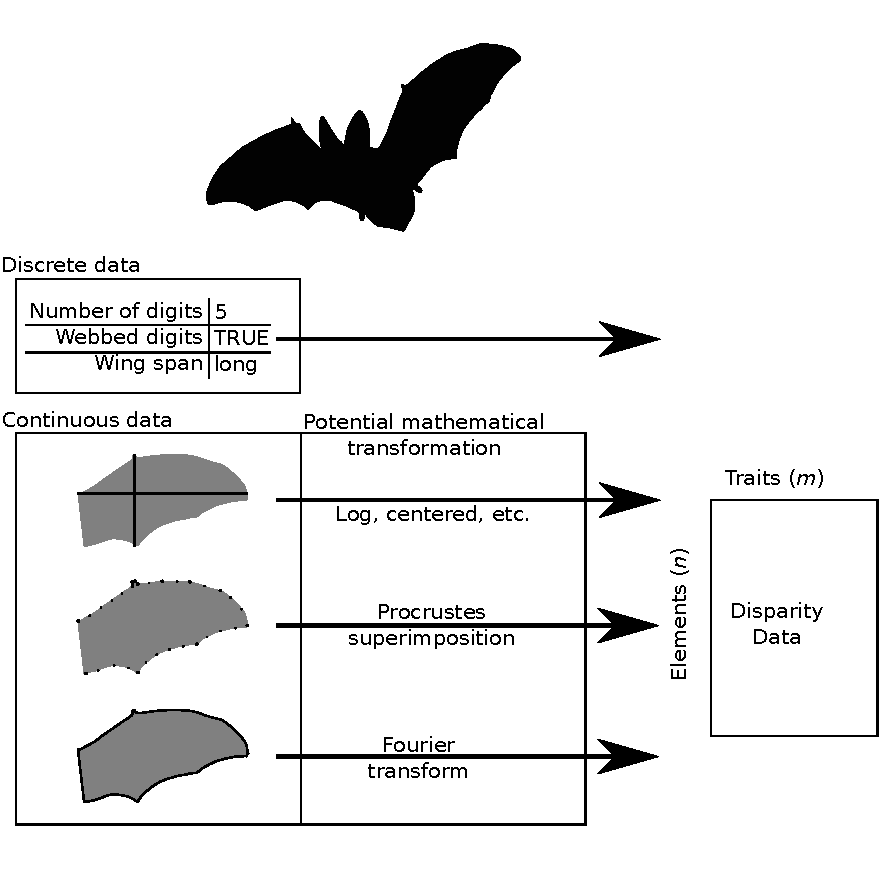
\includegraphics[width=0.9\textwidth]{Figures/figure_data.pdf}
\caption{
    Major routes to obtain morphological data for disparity analyses. Data can be collected as discrete trait observations (e.g. presence or absence data) or as continuous data.
    Continuous data can be collected by various methods including linear measurements and landmark coordinates or contours (curves).
    These measurements can then be mathematically transformed (logarithm transforms, scaling, Procrustes superimposition, elliptic Fourier transforms, etc.).
    Regardless of the method, data collection produces a trait matrix where the observed traits constitute columns and the studied elements (generally taxa or OTUs) the rows.
}
\label{Fig:data}
\end{figure}

\section{Disparity analysis methods}

\noindent Once suitable trait data have been collected, the design of the disparity analysis itself needs to be considered.
Study design encompasses several key aspects including (a) the difficulty of dealing with multidimensional data; (b) the variety of ordination (dimension reduction) techniques available and their limitations; (c) the metrics used to summarise the relative disparity of groups; (d) the methods used for hypothesis testing within the disparity analysis framework; and (e) ancestral state estimations in disparity-through-time analyses.
% @@@ Check the numbering here
We consider these aspects in turn below.









\subsection{a) To ordinate or not to ordinate - that is the (multidimensional) question}

% -Disparity analysis have a history of using ordination techniques
Disparity analyses often use ordination techniques for dimension reduction.
Dimension reduction (or ordination) is a powerful tool for visualizing data distribution in disparity analyses, helping to elucidate the underlying structure within datasets.
%     -Ordination techniques are blablabla
These are statistical methods to rearrange observed variables so that similar observations are closer together than dissimilar ones (e.g. principal component analysis -- PCA; principal coordinates analysis -- PCO/PCoA; non-metric multidimensional scaling -- NMDS; etc.).
Ordination techniques come in many flavours depending on the data and the desired morphospace properties.
Quantitative (continuous) data can be reduced using PCA, and qualitative data (or mixed data types) can be reduced using PCoA, which is equivalent to metric multidimensional scaling (MDS) or non-metric multidimensional scaling (NMDS) (see Legendre and Legendre 2012,chapter 9, for a detailed explanation of ordination methods and properties).
% -But mainly ordination is good for visualising.
Ordination is advantageous for plotting and visualising data, and can reveal properties of the morphospace not intuitively captured by disparity metrics (see Metrics section below {[}metrics{]}).
% -Ordination can be good for reducing dimensions if the data has a lot of measurements for a few number of observations (e.g. landmark data, discrete morphological characters, etc.)
Using ordinations in disparity analysis makes it easier for researchers to comprehend patterns in just two or three spatial dimensions at a time - or, indeed, just the first few axes of a PCA or a PCO.
Additionally, after ordinating the data, it is possible to reduce further the number of dimensions by focussing on just a subset of axes (e.g. selecting only those axes that describe the majority of the variation) or by fitting the variation to a prescribed number of axes.
In the case of geometric morphometric data, ordination is particularly useful as it conserves the mathematical properties of the data while efficiently reducing the dimensions (Legendre and Legendre 2012). %TG: cite also: Dryden and Mardia "Statistical Shape Analysis book"
This has clear advantages for interpreting the results.
For example, the axes will represent gradients of biological variation (e.g. elongation and flattening of the beak in birds \citep{Cooney2017-ly}.


% -However ordination can be problematic
However, like most other aspects of disparity analyses, reducing dimensionality can be tricky.
However, there are a number of potential problems with these transformations of the data.
%TG: comment from Sylvain: difference between a morphospace and an ordination space
%TG: comment from Graeme: the ordination space is decided by the data present (e.g. shoebill)
%     -It should contain all axis
In the case of ordination in a geometric morphometric context, subsampling axes from the ordination can lead to misinterpretation of the results. %TG: from Anjali: add that people should use 95% or 99% percent of the data (why not 100% though?)
%     -It is hard to interpret
Unfortunately, dimension reduction can introduce errors of interpretation when these principal axes are unrepresentative of the data more generally \citep{Bookstein1997-dn, Bookstein2015-yy, Bookstein2017-qk, Bookstein2017-gu,Weisbecker2019-kp}.
 %TG: Should be Bookstein 1991 "morphometric tools for landmark data" for the first reference
Visual interpretations of multidimensional data can be particularly misleading, not least since multidimensional spaces are not necessarily Euclidean even when analysing morphometric data \citep{Deline2018-le, Gerber2017-xi}.
Furthermore, interpreting biological variation along the axes is always a \textit{post-hoc} procedure and may have little relation to the overall question; for example, if the first few ordination axes represent the elongation of the beak in birds, but the question is about wing disparity.
Additionally, in some cases, reducing the dimensionality of a dataset can render its interpretation more problematic.
For example, when the analysed data is non-Euclidean (e.g. some types of discrete morphological characters such as inapplicable characters), interpreting the resulting ordinated space can be challenging, even if applying an ordination technique is straightforward, \citep{Gerber2017-xi}. %@@@TG: should be Gerber 2019
This is problematic when comparing the position of groups in multidimensional space, as the distances might not be linear.
Finally, \textit{post-hoc} interpretations of the gradient of variation on the ordination axes may be biologically meaningless or simply impossible. %TG: Cite Gerber 2019 10.1111/pala.12407
Although some gradients are easy to detect or interpret (e.g. the elongation and depth of mandibles in fishes on first and second PC axes, respectively; \citealt{Hill2018-ye}), some are not \citep[][e.g.]{Weisbecker2019-kp}.
For example, with discrete morphological data, a gradient between the species that have many characters in state 1 and the ones that have more in state 0, has no biological meaning if these are binary alternate states.
%     -It can make non-metric spaces
Categorical data are a good deal more problematic, since the characters themselves are invariably non-equivalent, non-independent, and mostly non-Euclidean and the distribution of the variance is usually normal (i.e. contrary to a PCA, the first few axis do not encompass most variance of the dataset).
Such non-Euclidean spaces often have non-intuitive properties, for example, straight lines viewed in bivariate plots of some two selected dimensions are not actually straight and, even less intuitively, distances are non-metric \citep[][i.e. the distance between A and B is not equal to the distance between B and A]{Gerber2014-ol}.
%     -It is often not necessary
And last but not least reason, In many cases, ordination might not be necessary.
For example, if a metric (e.g. sum or ranges of variance) used to characterise disparity can use all of the data (see Metrics section below metrics%indices
), it is not necessary to calculate it on ordinated data \citep{Close2015-qi}.
% -Disparity can be measured directly from the non-ordinated dataset (e.g. via distance matrices)
For all of these reasons, multidimensional data analyses should not be ordinated automatically, and careful consideration should be given to whether the aim of the study can be achieved without ordination \citep{lloyd2016,lloyd2018}.


% \hypertarget{a-multidimensionality}{%
% \subsection{(a) Multidimensionality}\label{a-multidimensionality}}

% Disparity analyses often use ordination techniques for dimension reduction.
% These are statistical methods to rearrange observed variables so that similar observations are closer together than dissimilar ones (e.g. principal component analysis -- PCA; principal coordinates analysis -- PCO/PCoA; non-metric multidimensional scaling -- NMDS; etc.).
% Using ordinations in disparity analysis makes it easier for researchers to comprehend patterns in just two or three spatial dimensions at a time - or, indeed, just the first few axes of a PCA or a PCO.
% Unfortunately, dimension reduction can introduce errors of interpretation when these principal axes are unrepresentative of the data more generally \href{https://paperpile.com/c/sTGYvp/1SD2+sN5d+xaUx+o4w7}{(}Bookstein \href{https://paperpile.com/c/sTGYvp/1SD2+sN5d+xaUx+o4w7}{1997, 2015, {[}b{]} 2017, {[}a{]} 2017)}{[}CITE Vera and Thomas paper{]}. %TG: Should be Bookstein 1991 "morphometric tools for landmark data" for the first reference
% Visual interpretations of multidimensional data can be particularly misleading, not least since multidimensional spaces are not necessarily Euclidean even when analysing morphometric data \href{https://paperpile.com/c/sTGYvp/0y4V+QVvv}{(Deline et al. 2018; Gerber 2017)}.
% Categorical data are a good deal more problematic, since the characters themselves are invariably non-equivalent, non-independent, and mostly non-Euclidean and the distribution of the variance is usually normal (i.e. contrary to a PCA, the first few axis do not encompass most variance of the dataset).
% Such non-Euclidean spaces often have non-intuitive properties, for example, straight lines viewed in bivariate plots of some two selected dimensions are not actually straight and, even less intuitively, distances are non-metric (\href{https://paperpile.com/c/sTGYvp/SJbC}{i.e. the distance between A and B is not equal to the distance between B and A; Gerber 2014)}.

% \hypertarget{b-to-ordinate-or-not-to-ordinate---that-is-the-multidimensional-question}{%
% \subsection{(b) To ordinate or not to ordinate - that is the
% (multidimensional)
% question}\label{b-to-ordinate-or-not-to-ordinate---that-is-the-multidimensional-question}}

% Dimension reduction (or ordination) is a powerful tool for visualizing data distribution in disparity analyses, helping to elucidate the underlying structure within datasets.
% However, like most other aspects of disparity analyses, reducing dimensionality can be tricky.
% Ordination techniques come in many flavours depending on the data and the desired morphospace properties.
% Quantitative (continuous) data can be reduced using PCA, and qualitative data (or mixed data types) can be reduced using PCoA, which is equivalent to metric multidimensional scaling (MDS) or non-metric multidimensional scaling (NMDS) (see Legendre and Legendre 2012,chapter 9, for a detailed explanation of ordination methods and properties).

% Ordination is advantageous for plotting and visualising data, and can reveal properties of the morphospace not intuitively captured by disparity metrics (see Metrics section below {[}metrics{]}).
% Additionally, after ordinating the data, it is possible to reduce further the number of dimensions by focussing on just a subset of axes (e.g. selecting only those axes that describe the majority of the variation) or by fitting the variation to a prescribed number of axes.
% In the case of geometric morphometric data, ordination is particularly useful as it conserves the mathematical properties of the data while efficiently reducing the dimensions (Legendre and Legendre 2012). %TG: cite also: Dryden and Mardia "Statistical Shape Analysis book"
% This has clear advantages for interpreting the results.
% For example, the axes will represent gradients of biological variation (e.g. elongation and flattening of the beak in birds \href{https://paperpile.com/c/sTGYvp/RjqE}{(Cooney et al. 2017}).
% However, there are a number of potential problems with these transformations of the data.
% %TG: comment from Sylvain: difference between a morphospace and an ordination space
% %TG: comment from Graeme: the ordination space is decided by the data present (e.g. shoebill)
% In the case of ordination in a geometric morphometric context, subsampling axes from the ordination can lead to misinterpretation of the results. %TG: from Anjali: add that people should use 95% or 99% percent of the data (why not 100% though?)
% Furthermore, interpreting biological variation along the axes is always a \emph{post-hoc} procedure and may have little relation to the overall question; for example, if the first few ordination axes represent the elongation of the beak in birds, but the question is about wing disparity.

% However, In many cases, ordination might not be necessary. For example, if a metric (e.g. sum or ranges of variance) used to characterise disparity can use all of the data (see Metrics section below {[}metrics{]}), it is not necessary to calculate it on ordinated data {[}e.g.\href{https://paperpile.com/c/sTGYvp/PbSx}{(Close et al. 2015)}{]}.
% Additionally, in some cases, reducing the dimensionality of a dataset can render its interpretation more problematic.
% For example, when the analysed data is non-Euclidean (e.g. some types of discrete morphological characters such as inapplicable characters), interpreting the resulting ordinated space can be challenging, even if applying an ordination technique is straightforward, \href{https://paperpile.com/c/sTGYvp/SJbC}{(}Gerber 2014\href{https://paperpile.com/c/sTGYvp/SJbC}{)}. %TG: should be Gerber 2019
% This is problematic when comparing the position of groups in multidimensional space, as the distances might not be linear.
% Finally, \emph{post-hoc} interpretations of the gradient of variation on the ordination axes may be biologically meaningless or simply impossible. %TG: Cite Gerber 2019 10.1111/pala.12407
% Although some gradients are easy to detect or interpret (e.g. the elongation and depth of mandibles in fishes on first and second PC axes, respectively; {[}\href{https://paperpile.com/c/sTGYvp/3JPy}{Hill et al. 2018{]}}), some are not (e.g. \href{https://paperpile.com/c/sTGYvp/TZzO}{Weisbecker et al. 2019)}.
% For example, with discrete morphological data, a gradient between the species that have many characters in state 1 and the ones that have more in state 0, has no biological meaning if these are binary alternate states.
% For all of these reasons, multidimensional data analyses should not be ordinated automatically, and careful consideration should be given to whether the aim of the study can be achieved without ordination (Lloyd 2016, 2018).









\begin{figure}[!htbp]
\centering
   \includegraphics[width=0.9\textwidth]{Figures/figure_space.pdf}
\caption{
    Morphospaces: different mathematical representations of a morphospace.
    % SG: The morphospace is the original trait space within which lie the specimens. Then one performs an ordination to visualize the space. So I would distinguish the morphospace from the ordination space. See also Mitteroecker and Huttegger (2009)
    A trait matrix can be transformed into a distance matrix \citep[][e.g in]{Close2015-qi} or an ordinated matrix \citep[][e.g. in]{Brusatte2008-vx}
    In each case, all three matrices represent the morphospace for the observations at hand.
    Visualisation: different ways to represent the morphospace in 2D.
    Visualisations can use either trait plots (directly from the trait matrix); ``flattening'' ordination of the data (e.g. using multidimensional scaling forcing all the variance to be contained in two dimensions)
    % SG: No, the flattening will not force all the variance to be contained in 2D. First because NMDS is non metric and variance is therefore not preserved as such. Second, because there is a stress associated with the flattening that correlates with the degree of distortion imposed on the data to enforce the 2D representation. Some information (variance) is thus necessarily lost.
    ; or ordination axis plots (directly from the ordinated matrix).
    % ES: I feel like somewhere we should say that in order for the spaces to be Euclidean, the axes must be on same scale. My little bugbear.
    % SG response: I think there are more conditions to be Euclidean (inner product defining the  Euclidean norm..). But surely if axes have different scales and units, it will be difficult to define a distance function and the space won't be metric.
    % @@@ Change references
}
\label{Fig:morphospace}
\end{figure}


% @@@ Change to indices throughout
\subsection{(b) Measuring disparity}

Most disparity datasets are multidimensional and, consequently, a large component of any disparity analysis involves considering how to extract a meaningful (i.e. interpretable) summary of disparity.
This is usually achieved with a disparity metric or index \citep{Hopkins2017-cf}.
As with any summary of multidimensional data, disparity metrics will reflect only some aspects of the morphological variation, never its whole complexity %metrics paper. CITE moms
It is therefore often beneficial to use more than one metric to summarise different aspects of variation, guided by the aim of the study.

When considering only one dimension, disparity metrics can be used to reflect the spread of the distribution (e.g. the range, quantiles or variance) or its central tendency (i.e., mean, median or mode).
Among these metrics, some will have more attractive properties than others, such as sensitivity to outliers. Range and mean are highly sensitive, whereas quantiles, variance and median are less so, making them more or less appropriate for different questions.
For example, if we want to characterise the extent of morphospace occupied by a group (e.g. does group A occupy as much space as group B?), metrics related to the spread of the group in the morphospace are most appropriate (e.g. volume
\citealt{Diaz2016-mr}, distance from the centroid \citealt{Hopkins2017-cf, Finlay2015-ft}, variance and range \citealt{Brusatte2008-fx}).
Conversely, if we wish to describe the ``position''
% SG: Note that conceptually and technically,  disparity is about variation. So information on position is another aspect of morphospace occupation. but it is distinct from the meaning of  disparity as originally intended.
 of a group in a morphospace (e.g. does group A occupy the same space as group B?), metrics related to the distance between the elements within a group and a fixed point in the morphospace are most appropriate. %@@@ CITE moms
Finally, if we aim to characterise the density of morphospace occupation (e.g. is group A more closely packed than group B?) metrics related to the pairwise distances between elements will be most appropriate (e.g. nearest neighbour distance, pairwise distances, etc. \citealt{Close2015-qi}).
%ES: this para is probably most useful to refer to for the ordinate or not part

In addition to considering what properties of disparity metrics should capture, it is important to also consider the mathematical properties of the metrics and their associated caveats \citep{Wills2001-wh, Ciampaglio2001-iz}.
For example, measuring the full sum of the variance in each dimension of the space does not require we add the covariance between the axes in an ordinated space using a PCA.
% SG: Not very clear to me
However, this is not true of other mathematical spaces or when not all dimensions or elements are considered, even in a PCA \citep{Legendre2012-va}.

Furthermore, multidimensional spaces also have some counter-intuitive properties that need to be considered such as the ``curse of dimensionality'' \citep{Bellman1966-mc}.
In spaces with some axis of variance lower than 1, product-based metrics used as proxies of volumes (e.g. product of ranges, hypervolume, hypercube, etc.) can tend towards zero fairly quickly for spaces with even a modest number of dimensions \citep{Bellman1966-mc}. %Donoho 2000
Some other types of metrics are also extremely sensitive to outliers and can be biased easily by sample size, for example range \citep{Butler2012-tr}
%SG: Or even better, twenty years earlier, Foote (1992), who orginally described the problem in the context of disparity and suggested a rarefaction approach.
or convex hull based metrics \citep{Butler2012-tr, Jackson2011-kq}.

\subsection{(c) Testing hypotheses on the evolution of
disparity}

No matter which disparity metrics have been calculated, the research question must be framed in an appropriate statistical context.
The multidimensional statistical toolkit for ecology and evolution has been greatly expanded in recent years \citep{Adams2018-mg}
%AG: there are others that should be mentioned - mvmorph for example, which is especially important given that there are extremely different approaches to multivariate data in these different packages
, but some of these advances have yet to be implemented in disparity analyses. Instead, hypothesis testing has mostly been confined to a small set of well-established methods.
One commonly used test is the non-parametric permutation analysis of variance \citep{Anderson2001-qb, Anderson2013-zt}, an analysis of variance (ANOVA) of the pairwise distances between different groups.
Although statistically valid, this test is not always directly related to the hypothesis under question.
For example, PERMANOVA tests whether two groups share the same variance/covariance in a ``distance-space''.
% SG: What is meant by distance-sapce and in what way is it distinguished from the spaces discussed above?
This is not the same as testing whether the two groups overlap in morphospace.
%SG: You're sure of this?
Statistical tests should be employed that are tailored to the question at hand, rather than simply following common practices.

It is also important to consider which data should be subjected to a statistical test.
% AG: It would be good to also note here that data should be comparable in terms of having a common reference frame - e.g. comparing disparities across elements with different numbers of landmarks or different landmark configurations that haven't been/can't be superimposed together is problematic but is popping up in the disparity literature
For example, in morphological disparity analysis, especially for palaeobiological questions, data are often bootstrapped.
This has two advantages: (i) when the disparity metric is unidimensional (e.g. the sum of variances), bootstrapping the data generates a distribution of the metric that can be analysed using the vast statistical toolkit available for comparing distributions; (ii) when data are scarce, bootstrapping the data allows users to introduce variance, rendering the test less sensitive to outliers.
However, bootstrapped data are pseudoreplicates and thus non-independent.
This violates the assumptions of most parametric statistical tests.
Furthermore, the number of bootstrap pseudoreplicates will inevitably increase the false positive rate (Type I error).
% @@@ check positive/negative type
These factors are often ignored in disparity analyses.
% VW: Surely there's a reference for this?
% MH: I might be wrong about this, but my impression is that CIs generated from bootstrapping are compared visually (like to assess significance in changes in disparity over time), but that statistical tests are not commonly applied.

%TG: Add section d) within c)
\subsection{(d) Phylogenetic autocorrelation}

As with all comparative datasets, the data used in disparity analyses are not independent because close relatives will tend to have more similar morphologies than more distant relatives \citep{Harvey1998-xg}.
Thus, for many disparity analyses, phylogenetic relationships should be
taken into account.
% SG: Why?
However, it has been noted that some popular phylogenetic correction methods (like pPCA) can be inappropriate
% SG: In what way?
if incorrect assumptions are made about the data \citep{Uyeda2015}.
% @@@ref: https://academic.oup.com/sysbio/article/64/4/677/1649888
% SG: Which assumption? This part (e) seems a bit vague to me
% AG: as long as you are using most or ideally all of the variance in a dataset, the rotation of pPCA should have little to no impact on disparity analyses. polly et al 2013 i think
provide a thorough review of multivariate phylogenetic comparative methods, and so we do not consider them further here.
% AG: Given this is given quite short treatment, i think if you need room, you could cut it altogether or just have a sentence in another section stating this even more briefly

%TG: Add section e) within c)???
\subsection{(e) Ancestral state estimation in disparity-through-time analyses}

Disparity-through-time analyses often use ancestral state estimation to extract disparity estimates for non-sampled taxa and/or nodes of a phylogeny.
Ancestral state estimation can be performed at two points in the disparity analysis pipeline: either (1) pre-ordination, i.e. the estimation is done before transformation of the data (e.g. ordination, or distance matrix construction) and is simply based on the original data; or (2) post-ordination, i.e. the estimation is done after transformation of the data by estimating the ancestral states using the transformed matrix (e.g. the ordination scores) \citep{lloyd2018}.

Pre-ordination ancestral state estimation will change the way the ordination space is defined -- i.e. the relationship between the points are not yet estimated -- and requires longer computational times.
However, once the morphospace is defined its properties will not change.
Post-ordination ancestral state estimation will not change the empirical ordination space and is faster to compute, but it will add elements in the space, whose estimated positions can be problematic for statistical tests and evolutionary inferences down the line \citep{lloyd2018}.

No ancestral state estimation method is without drawbacks
% @@@ Maybe check in Pennel’s “fossils are needed” paper for ref.
 and above all else are highly dependent on the data and method used.
In general, using ancestral state estimation can help with recovering patterns of changes in disparity but should not be used simply to generate extra data points to increase statistical power.
In fact, these extra points are not independent and can also have problematic side effects, especially when testing for the influence of mass extinctions on disparity.

\section{Disparity analyses for the future}

\noindent Morphological disparity analyses are widely employed in evolutionary palaeobiology, and they are based on a diversity of methods and data.
There is no ``one-size-fits-all'' pipeline for morphological disparity analyses.
As with any multidimensional analysis, there are many variables that have to be considered when deciding which data to use and how to analyse it, stemming from the explicit hypotheses being tested.
Many of the problems in morphological disparity analysis arise from ``blind'' application of established methodological pipelines without consideration of the biological question being addressed.
We advocate the bespoke
%VW: I think there could be just a line or two that takes makes "bespoke design" less daunting. There are loads of well-documented R packages available in morphological and ecological studies that can be relatively straightforwardly adapted.
assembly of analytic approaches and, given the computational efficiency of these methods, an experimental approach that explores the impact of competing approaches, such as choice of distance measure, ordination method and ancestral state estimation method on disparity analysis results.
Many of the methods employed in disparity analysis are used more widely in other fields, including genomics and ecology, which also encompass analyses of multidimensional datasets
\citep{Donohue2013-bg, Saupe2015-vm, Canter2018-hk, mammola2019}
. % @@@ Add Mammola
Innovations in morphological disparity analyses likely await discovery in their respective literatures.
% AG: as above, i think you need to add in evodevo work here, it's really fundamental to disparity

While studies of morphological disparity would benefit from advances in multidimensional analysis in other fields, the concept of a morphospace could reciprocally benefit other disciplines.
For example, the multidimensional analysis of Diaz \citealt{Diaz2016-mr}, which analysed patterns of form and function in plants, is essentially an ecomorphospace; isotopic analyses of organisms \citep{Jackson2011-kq} can be represented as an isotope-space; ecosystem functioning in \citealt{Donohue2013-bg} as an ecosystem-space, etc.
% AJ: this is a potential nice, although rather data hungry I believe, methods that I think could be worth dropping into the paper somewhere. Either here as a quick drop, or earlier up under overlap seems appropriate if you want to add it https://esajournals.onlinelibrary.wiley.com/doi/10.1890/14-0235.1
These generalisations could also be exported for any set of traits (e.g. acousto-spaces for acoustic traits or glotto-spaces for linguistic traits).
%SG: devising 
Cognate approaches have been adopted recently in the analysis of single cell comparative transcriptome data \citep{Sebe-Pedros2018-sw} where interpretation of the resulting transcriptome-spaces would be improved by heeding the concerns we highlight concerning morphospaces.
% ES: Suggested by Erin: reword this sentence

Although disparity analyses are now simple to implement in freely available softwares \citep{Navarro2003-vz, Bouxin2005-wk, oksanen2007vegan, Harmon2008-gq, lloyd2016, Guillerme2018-uc}.
it is crucial to remember that they are multidimensional analyses and multidimensional analyses are complex.
We assert that future morphological analyses will benefit by emphasising the methodological decisions made, rather than simply using disparity analysis because \textit{we can}.

\subsection{Author contributions}

TG, NC and PD proposed this review; TG and NC led the writing supported by PD and GT. All authors edited drafts and approved the final version.

\subsection{Acknowledgements}

This article results from discussion at the Royal Society International Science Seminar on `Reconciling disparate views on disparity' held at Chicheley Hall, 9-10th January, 2018.

-AG was funded by European Research Council Starting grant 637171 ADaPTiVE.

-ALJ was funded by an Irish Research Council Laureate Award IRCLA/2017/186. ES was funded by a University of Adelaide Research Fellowship;

-EES was funded by a Leverhulme Trust Research Project Grant (DGR01020).

-PD was funded by NERC (NE/P013678/1; NE/N002067/1) and BBSRC (BB/N000919/1);

-SB was funded by European Research Council (ERC) under the European Union's Horizon 2020 research and innovation program (grant agreement No 756226, ERC Starting Grant: PalM) and a Leverhulme Trust Research Project Grant (RPG-2017-167);

-TG was funded by ARC DP170103227 and FT180100634 awarded to VW;


\bibliographystyle{sysbio}
\bibliography{References}


\end{document}
















% Donoho, D. L. (2000). High-dimensional data analysis: The curses and
% blessings of dimensionality. \emph{AMS math challenges lecture},
% \emph{1}(2000), 32.

% References

% \href{http://paperpile.com/b/sTGYvp/ZnDd}{Adams, Dean C., and Michael L.
% Collyer. 2018. ``Multivariate Phylogenetic Comparative Methods:
% Evaluations, Comparisons, and Recommendations.'' \emph{Systematic
% Biology} 67 (1): 14--31.}

% \href{http://paperpile.com/b/sTGYvp/J2G1}{Adams, Dean C., and Erik
% Otárola-Castillo. 2013. ``Geomorph: Anrpackage for the Collection and
% Analysis of Geometric Morphometric Shape Data.'' \emph{Methods in
% Ecology and Evolution / British Ecological Society} 4 (4): 393--99.}

% \href{http://paperpile.com/b/sTGYvp/SC6L}{Anderson, Marti J. 2001. ``A
% New Method for Non-Parametric Multivariate Analysis of Variance.''
% \emph{Austral Ecology} 26 (1): 32--46.}

% \href{http://paperpile.com/b/sTGYvp/3hy2}{Anderson, Marti J., and Daniel
% C. I. Walsh. 2013. ``PERMANOVA, ANOSIM, and the Mantel Test in the Face
% of Heterogeneous Dispersions: What Null Hypothesis Are You Testing?''
% \emph{Ecological Monographs} 83 (4): 557--74.}

% \href{http://paperpile.com/b/sTGYvp/qjj9}{Anderson, Philip S. L., Matt
% Friedman, Martin D. Brazeau, and Emily J. Rayfield. 2011. ``Initial
% Radiation of Jaws Demonstrated Stability despite Faunal and
% Environmental Change.'' \emph{Nature} 476 (7359): 206--9.}

% \href{http://paperpile.com/b/sTGYvp/Qsl3}{Bellman, R. 1966. ``Dynamic
% Programming.'' \emph{Science} 153 (3731): 34--37.}

% \href{http://paperpile.com/b/sTGYvp/1SD2}{Bookstein, Fred L. 1997.
% \emph{Morphometric Tools for Landmark Data: Geometry and Biology}.
% Cambridge University Press.}

% \href{http://paperpile.com/b/sTGYvp/sN5d}{---------. 2015. ``The
% Relation between Geometric Morphometrics and Functional Morphology, as
% Explored by Procrustes Interpretation of Individual Shape Measures
% Pertinent to Function.'' \emph{Anatomical Record} 298 (1): 314--27.}

% \href{http://paperpile.com/b/sTGYvp/o4w7}{---------. 2017a. ``A Newly
% Noticed Formula Enforces Fundamental Limits on Geometric Morphometric
% Analyses.'' \emph{Evolutionary Biology} 44 (4): 522--41.}

% \href{http://paperpile.com/b/sTGYvp/xaUx}{---------. 2017b. ``A Method
% of Factor Analysis for Shape Coordinates.'' \emph{American Journal of
% Physical Anthropology} 164 (2): 221--45.}

% \href{http://paperpile.com/b/sTGYvp/9JdS}{Bouxin, Guy. 2005. ``Ginkgo, a
% Multivariate Analysis Package.'' \emph{Journal of Vegetation Science:
% Official Organ of the International Association for Vegetation Science}
% 16 (3): 355--59.}

% \href{http://paperpile.com/b/sTGYvp/Yrbg}{Brazeau, Martin D., Thomas
% Guillerme, and Martin R. Smith. 2017. ``Morphological Phylogenetic
% Analysis with Inapplicable Data.''
% https://doi.org/}\href{http://dx.doi.org/10.1101/209775}{10.1101/209775}\href{http://paperpile.com/b/sTGYvp/Yrbg}{.}

% \href{http://paperpile.com/b/sTGYvp/tGyd}{Brusatte, S. L., M. J. Benton,
% M. Ruta, and G. T. Lloyd. 2008. ``The First 50 Myr of Dinosaur
% Evolution: Macroevolutionary Pattern and Morphological Disparity.''
% \emph{Biology Letters} 4 (6): 733--36.}

% \href{http://paperpile.com/b/sTGYvp/EeC8}{Brusatte, Stephen L., Michael
% J. Benton, Marcello Ruta, and Graeme T. Lloyd. 2008. ``Superiority,
% Competition, and Opportunism in the Evolutionary Radiation of
% Dinosaurs.'' \emph{Science} 321 (5895): 1485--88.}

% \href{http://paperpile.com/b/sTGYvp/aSSL}{Butler, Richard J., Stephen L.
% Brusatte, Brian Andres, and Roger B. J. Benson. 2012. ``How Do
% Geological Sampling Biases Affect Studies of Morphological Evolution in
% Deep Time? A Case Study of Pterosaur (Reptilia: Archosauria)
% Disparity.'' \emph{Evolution; International Journal of Organic
% Evolution} 66 (1): 147--62.}

% \href{http://paperpile.com/b/sTGYvp/60H0}{Canter, Erin J., Catalina
% Cuellar-Gempeler, Abigail I. Pastore, Thomas E. Miller, and Olivia U.
% Mason. 2018. ``Predator Identity More than Predator Richness Structures
% Aquatic Microbial Assemblages in Sarracenia Purpurea Leaves.''
% \emph{Ecology} 99 (3): 652--60.}

% \href{http://paperpile.com/b/sTGYvp/ROH8}{Ciampaglio, Charles N.,
% Matthieu Kemp, and Daniel W. McShea. 2001. ``Detecting Changes in
% Morphospace Occupation Patterns in the Fossil Record: Characterization
% and Analysis of Measures of Disparity.'' \emph{Paleobiology} 27 (4):
% 695--715.}

% \href{http://paperpile.com/b/sTGYvp/PbSx}{Close, Roger A., Matt
% Friedman, Graeme T. Lloyd, and Roger B. J. Benson. 2015. ``Evidence for
% a Mid-Jurassic Adaptive Radiation in Mammals.'' \emph{Current Biology:
% CB} 25 (16): 2137--42.}

% \href{http://paperpile.com/b/sTGYvp/RjqE}{Cooney, Christopher R., Jen A.
% Bright, Elliot J. R. Capp, Angela M. Chira, Emma C. Hughes, Christopher
% J. A. Moody, Lara O. Nouri, Zoë K. Varley, and Gavin H. Thomas. 2017.
% ``Mega-Evolutionary Dynamics of the Adaptive Radiation of Birds.''
% \emph{Nature} 542 (7641): 344--47.}

% \href{http://paperpile.com/b/sTGYvp/0y4V}{Deline, Bradley, Jennifer M.
% Greenwood, James W. Clark, Mark N. Puttick, Kevin J. Peterson, and
% Philip C. J. Donoghue. 2018. ``Evolution of Metazoan Morphological
% Disparity.'' \emph{Proceedings of the National Academy of Sciences of
% the United States of America} 115 (38): E8909--18.}

% \href{http://paperpile.com/b/sTGYvp/47fI}{Díaz, Sandra, Jens Kattge,
% Johannes H. C. Cornelissen, Ian J. Wright, Sandra Lavorel, Stéphane
% Dray, Björn Reu, et al. 2016. ``The Global Spectrum of Plant Form and
% Function.'' \emph{Nature} 529 (7585): 167--71.}

% \href{http://paperpile.com/b/sTGYvp/2KmX}{Dixon, Philip. 2003. ``VEGAN,
% a Package of R Functions for Community Ecology.'' \emph{Journal of
% Vegetation Science: Official Organ of the International Association for
% Vegetation Science} 14 (6): 927.}

% \href{http://paperpile.com/b/sTGYvp/krNU}{Donohue, Ian, Owen L. Petchey,
% José M. Montoya, Andrew L. Jackson, Luke McNally, Mafalda Viana, Kevin
% Healy, Miguel Lurgi, Nessa E. O'Connor, and Mark C. Emmerson. 2013. ``On
% the Dimensionality of Ecological Stability.'' \emph{Ecology Letters} 16
% (4): 421--29.}

% \href{http://paperpile.com/b/sTGYvp/EPJ2}{Erwin, Douglas H. 2007.
% ``DISPARITY: MORPHOLOGICAL PATTERN AND DEVELOPMENTAL CONTEXT.''
% \emph{Palaeontology}.
% https://doi.org/}\href{http://dx.doi.org/10.1111/j.1475-4983.2006.00614.x}{10.1111/j.1475-4983.2006.00614.x}\href{http://paperpile.com/b/sTGYvp/EPJ2}{.}

% \href{http://paperpile.com/b/sTGYvp/Z6l6}{---------. 2011.
% ``Evolutionary Uniformitarianism.'' \emph{Developmental Biology} 357
% (1): 27--34.}

% \href{http://paperpile.com/b/sTGYvp/yyNa}{Finlay, Sive, and Natalie
% Cooper. 2015. ``Morphological Diversity in Tenrecs (Afrosoricida,
% Tenrecidae): Comparing Tenrec Skull Diversity to Their Closest
% Relatives.'' \emph{PeerJ} 3 (April): e927.}

% \href{http://paperpile.com/b/sTGYvp/2Neu}{Foote, Mike. 1989.
% ``Perimeter-Based Fourier Analysis: A New Morphometric Method Applied to
% the Trilobite Cranidium.'' \emph{Journal of Paleontology}.
% https://doi.org/}\href{http://dx.doi.org/10.1017/s0022336000036556}{10.1017/s0022336000036556}\href{http://paperpile.com/b/sTGYvp/2Neu}{.}

% \href{http://paperpile.com/b/sTGYvp/fTJ3}{---------. 1995.
% ``Morphological Diversification of Paleozoic Crinoids.''
% \emph{Paleobiology} 21 (03): 273--99.}

% \href{http://paperpile.com/b/sTGYvp/yqPw}{---------. 1997. ``THE
% EVOLUTION OF MORPHOLOGICAL DIVERSITY.'' \emph{Annual Review of Ecology
% and Systematics} 28 (1): 129--52.}

% \href{http://paperpile.com/b/sTGYvp/2tbJ}{Fortey, R. A., D. E. G.
% Briggs, and M. A. Wills. 1996. ``The Cambrian Evolutionary `explosion':
% Decoupling Cladogenesis from Morphological Disparity.'' \emph{Biological
% Journal of the Linnean Society. Linnean Society of London} 57 (1):
% 13--33.}

% \href{http://paperpile.com/b/sTGYvp/EETc}{Friedman, Matt. 2010.
% ``Explosive Morphological Diversification of Spiny-Finned Teleost Fishes
% in the Aftermath of the End-Cretaceous Extinction.'' \emph{Proceedings.
% Biological Sciences / The Royal Society} 277 (1688): 1675--83.}

% \href{http://paperpile.com/b/sTGYvp/SJbC}{Gerber, Sylvain. 2014. ``Not
% All Roads Can Be Taken: Development Induces Anisotropic Accessibility in
% Morphospace.'' \emph{Evolution \& Development} 16 (6): 373--81.}

% \href{http://paperpile.com/b/sTGYvp/QVvv}{---------. 2017. ``The
% Geometry of Morphospaces: Lessons from the Classic Raup Shell Coiling
% Model.'' \emph{Biological Reviews of the Cambridge Philosophical
% Society} 92 (2): 1142--55.}

% \href{http://paperpile.com/b/sTGYvp/Uns3}{Gould, Stephen Jay. 2000.
% \emph{Wonderful Life: The Burgess Shale and the Nature of History}.
% Random House.}

% \href{http://paperpile.com/b/sTGYvp/xDqf}{Guillerme, Thomas. 2018.
% ``dispRity : A Modular R Package for Measuring Disparity.''
% \emph{Methods in Ecology and Evolution / British Ecological Society} 9
% (7): 1755--63.}

% \href{http://paperpile.com/b/sTGYvp/ekU4}{Guillerme, Thomas, and Natalie
% Cooper. 2018. ``Time for a Rethink: Time Sub-Sampling Methods in
% Disparity-through-Time Analyses.'' \emph{Palaeontology} 61 (4):
% 481--93.}

% \href{http://paperpile.com/b/sTGYvp/u1KE}{Guillerme, Thomas, Mark N.
% Puttick, Ariel E. Marcy, and Vera Weisbecker. n.d. ``Shifting Spaces:
% Which Disparity or Dissimilarity Metrics Best Summarise Occupancy in
% Multidimensional Spaces?''
% https://doi.org/}\href{http://dx.doi.org/10.1101/801571}{10.1101/801571}\href{http://paperpile.com/b/sTGYvp/u1KE}{.}

% \href{http://paperpile.com/b/sTGYvp/9Zoi}{Harmon, Luke J., Jason T.
% Weir, Chad D. Brock, Richard E. Glor, and Wendell Challenger. 2008.
% ``GEIGER: Investigating Evolutionary Radiations.'' \emph{Bioinformatics}
% 24 (1): 129--31.}

% \href{http://paperpile.com/b/sTGYvp/WXik}{Harvey, Paul H., and Mark D.
% Pagel. 1998. \emph{The Comparative Method in Evolutionary Biology}.
% Oxford University Press, USA.}

% \href{http://paperpile.com/b/sTGYvp/3JPy}{Hill, Jennifer J., Mark N.
% Puttick, Thomas L. Stubbs, Emily J. Rayfield, and Philip C. J. Donoghue.
% 2018. ``Evolution of Jaw Disparity in Fishes.'' \emph{Palaeontology}.
% https://doi.org/}\href{http://dx.doi.org/10.1111/pala.12371}{10.1111/pala.12371}\href{http://paperpile.com/b/sTGYvp/3JPy}{.}

% \href{http://paperpile.com/b/sTGYvp/xLdm}{Hopkins, Melanie J. 2017.
% ``How Well Does a Part Represent the Whole? A Comparison of Cranidial
% Shape Evolution with Exoskeletal Character Evolution in the Trilobite
% Family Pterocephaliidae.'' \emph{Palaeontology} 60 (3): 309--18.}

% \href{http://paperpile.com/b/sTGYvp/vTHS}{Hopkins, Melanie J., and
% Sylvain Gerber. 2017. ``Morphological Disparity.'' In \emph{Evolutionary
% Developmental Biology}, 1--12.}

% \href{http://paperpile.com/b/sTGYvp/hea5}{Hopkins, M. J. 2013.
% ``Decoupling of Taxonomic Diversity and Morphological Disparity during
% Decline of the Cambrian Trilobite Family Pterocephaliidae.''
% \emph{Journal of Evolutionary Biology} 26 (8): 1665--76.}

% \href{http://paperpile.com/b/sTGYvp/xxh5}{Hughes, Martin, Sylvain
% Gerber, and Matthew Albion Wills. 2013. ``Clades Reach Highest
% Morphological Disparity Early in Their Evolution.'' \emph{Proceedings of
% the National Academy of Sciences of the United States of America} 110
% (34): 13875--79.}

% \href{http://paperpile.com/b/sTGYvp/PwyQ}{Jackson, Andrew L., Richard
% Inger, Andrew C. Parnell, and Stuart Bearhop. 2011. ``Comparing Isotopic
% Niche Widths among and within Communities: SIBER - Stable Isotope
% Bayesian Ellipses in R.'' \emph{The Journal of Animal Ecology} 80 (3):
% 595--602.}

% \href{http://paperpile.com/b/sTGYvp/oFiP}{Legendre, P., and Loic F. J.
% Legendre. 2012. \emph{Numerical Ecology}. Elsevier.}

% \href{http://paperpile.com/b/sTGYvp/bCsU}{Lloyd, Graeme T. 2016.
% ``Estimating Morphological Diversity and Tempo with Discrete
% Character-Taxon Matrices: Implementation, Challenges, Progress, and
% Future Directions.'' \emph{Biological Journal of the Linnean Society.
% Linnean Society of London} 118 (1): 131--51.}

% \href{http://paperpile.com/b/sTGYvp/53SJ}{---------. 2018. ``Journeys
% through Discrete-Character Morphospace: Synthesizing Phylogeny, Tempo,
% and Disparity.'' \emph{Palaeontology} 61 (5): 637--45.}

% \href{http://paperpile.com/b/sTGYvp/dJHu}{Losos, Jonathan B. 2011.
% \emph{Lizards in an Evolutionary Tree: Ecology and Adaptive Radiation of
% Anoles}. Univ of California Press.}

% \href{http://paperpile.com/b/sTGYvp/aVVj}{Moyne, Sébastien, and Pascal
% Neige. 2007. ``The Space-Time Relationship of Taxonomic Diversity and
% Morphological Disparity in the Middle Jurassic Ammonite Radiation.''
% \emph{Palaeogeography, Palaeoclimatology, Palaeoecology} 248 (1-2):
% 82--95.}

% \href{http://paperpile.com/b/sTGYvp/EmTR}{Navarro, Nicolas. 2003. ``MDA:
% A MATLAB-Based Program for Morphospace-Disparity Analysis.''
% \emph{Computers \& Geosciences} 29 (5): 655--64.}

% \href{http://paperpile.com/b/sTGYvp/yO2t}{Palci, Alessandro, and Michael
% S. Y. Lee. 2018. ``Geometric Morphometrics, Homology and Cladistics:
% Review and Recommendations.'' \emph{Cladistics: The International
% Journal of the Willi Hennig Society}.
% https://doi.org/}\href{http://dx.doi.org/10.1111/cla.12340}{10.1111/cla.12340}\href{http://paperpile.com/b/sTGYvp/yO2t}{.}

% \href{http://paperpile.com/b/sTGYvp/tSIy}{Pierce, Stephanie E., Kenneth
% D. Angielczyk, and Emily J. Rayfield. 2008. ``Patterns of Morphospace
% Occupation and Mechanical Performance in Extant Crocodilian Skulls: A
% Combined Geometric Morphometric and Finite Element Modeling Approach.''
% \emph{Journal of Morphology} 269 (7): 840--64.}

% \href{http://paperpile.com/b/sTGYvp/I0Ic}{Raup, D. M. 1961. ``THE
% GEOMETRY OF COILING IN GASTROPODS.'' \emph{Proceedings of the National
% Academy of Sciences of the United States of America} 47 (4): 602--9.}

% \href{http://paperpile.com/b/sTGYvp/geAO}{Ruta, Marcello, Kenneth D.
% Angielczyk, Jörg Fröbisch, and Michael J. Benton. 2013. ``Decoupling of
% Morphological Disparity and Taxic Diversity during the Adaptive
% Radiation of Anomodont Therapsids.'' \emph{Proceedings. Biological
% Sciences / The Royal Society} 280 (1768): 20131071.}

% \href{http://paperpile.com/b/sTGYvp/cV3v}{Saupe, Erin E., Huijie Qiao,
% Jonathan R. Hendricks, Roger W. Portell, Stephen J. Hunter, Jorge
% Soberón, and Bruce S. Lieberman. 2015. ``Niche Breadth and Geographic
% Range Size as Determinants of Species Survival on Geological Time
% Scales.'' \emph{Global Ecology and Biogeography}.
% https://doi.org/}\href{http://dx.doi.org/10.1111/geb.12333}{10.1111/geb.12333}\href{http://paperpile.com/b/sTGYvp/cV3v}{.}

% \href{http://paperpile.com/b/sTGYvp/856K}{Sebé-Pedrós, Arnau, Elad
% Chomsky, Kevin Pang, David Lara-Astiaso, Federico Gaiti, Zohar Mukamel,
% Ido Amit, Andreas Hejnol, Bernard M. Degnan, and Amos Tanay. 2018.
% ``Early Metazoan Cell Type Diversity and the Evolution of Multicellular
% Gene Regulation.'' \emph{Nature Ecology \& Evolution} 2 (7): 1176--88.}

% \href{http://paperpile.com/b/sTGYvp/ZEDR}{Spriggs, Elizabeth L., Samuel
% B. Schmerler, Erika J. Edwards, and Michael J. Donoghue. 2018. ``Leaf
% Form Evolution in Viburnum Parallels Variation within Individual
% Plants.'' \emph{The American Naturalist} 191 (2): 235--49.}

% \href{http://paperpile.com/b/sTGYvp/Ejzr}{Wainwright, Peter C., Michael
% E. Alfaro, Daniel I. Bolnick, and C. Darrin Hulsey. 2005. ``Many-to-One
% Mapping of Form to Function: A General Principle in Organismal Design?''
% \emph{Integrative and Comparative Biology} 45 (2): 256--62.}

% \href{http://paperpile.com/b/sTGYvp/TZzO}{Weisbecker, Vera, Thomas
% Guillerme, Cruise Speck, Emma Sherratt, Hyab Mehari Abraha, Alana C.
% Sharp, Claire E. Terhune, Simon Collins, Stephen Johnston, and Olga
% Panagiotopoulou. 2019. ``Individual Variation of the Masticatory System
% Dominates 3D Skull Shape in the Herbivory-Adapted Marsupial Wombats.''
% \emph{Frontiers in Zoology} 16 (November): 41.}

% \href{http://paperpile.com/b/sTGYvp/nFf7}{Wills, Matthew A. 2001.
% ``Morphological Disparity: A Primer.'' In \emph{Topics in Geobiology},
% 55--144.}

% \href{http://paperpile.com/b/sTGYvp/eZ3F}{Wills, Matthew A., Derek E. G.
% Briggs, and Richard A. Fortey. 1994. ``Disparity as an Evolutionary
% Index: A Comparison of Cambrian and Recent Arthropods.''
% \emph{Paleobiology} 20 (02): 93--130.}

% \href{http://paperpile.com/b/sTGYvp/s33b}{Wright, David F. 2017.
% ``Phenotypic Innovation and Adaptive Constraints in the Evolutionary
% Radiation of Palaeozoic Crinoids.'' \emph{Scientific Reports} 7 (1):
% 13745.}
